\documentclass{article}
\linespread{1.25}

\usepackage{amsmath}
\usepackage[top = 1cm, right=2cm, left=2cm]{geometry}
\usepackage{tikz}
\usepackage{graphicx}
\usepackage{xepersian}
\settextfont{B Nazanin}
\setlatinmonofont{CMU Serif}
%\setlatinmonofont{Times New Roman}
\setlatintextfont{Times New Roman}

% Set Latin Modern font for the bullets in itemizea
\newfontfamily\latinbullet{Latin Modern Roman}



\title{پاسخ تکلیف مبحث
	\lr{Concept Learning}
}
\author{درس یادگیری ماشین}
\date{
	امیرحسین ابوالحسنی\\
	400405003
	}
	
	
% Commands
\newcommand{\column}[1]{\lr{\textit{#1}}}
\renewcommand{\labelitemi}{{\latinbullet\textbullet}} % Use the bullet from Latin Modern font

\newcommand{\ap}[3]{\draw (#1,#2) node[scale=2] {#3};}
\newcommand{\mkrect}[5][black]{% #1: optional color, #2: x1, #3: y1, #4: x2, #5: y2
	\draw[#1,very thick] (#2,#3) rectangle (#4,#5);
}

\begin{document}
	\maketitle
	
	\begin{latin}
		\section{Consider the instance space consisting of integer points in the $x$ , $y$ plane and the
			set of hypotheses $H$ consisting of rectangles.\\
			More precisely,\\
			hypotheses are of the
			form $a \le x \le b$, $c \le y \le d$ , where $a , b, c,$ and $d$ can be any integers.}
			
			% Q1-a
			\subsection{Consider the version space with respect to the set of positive ($+$) and negative
				($-$) training examples shown below. What is the $S$ boundary of the version space
				in this case? Write out the hypotheses and draw them in on the diagram.}
				
				% S boundry
				\subsubsection*{Answer:}			
				$$
				S = \{h\}
				$$
				$$
				h: 4 \le x \le 6 ~~ , ~~ 3 \le y \le 5
				$$
				The \textit{red} rectangle is the $S$ boundary :
						\begin{figure}[h!]
							\centering
							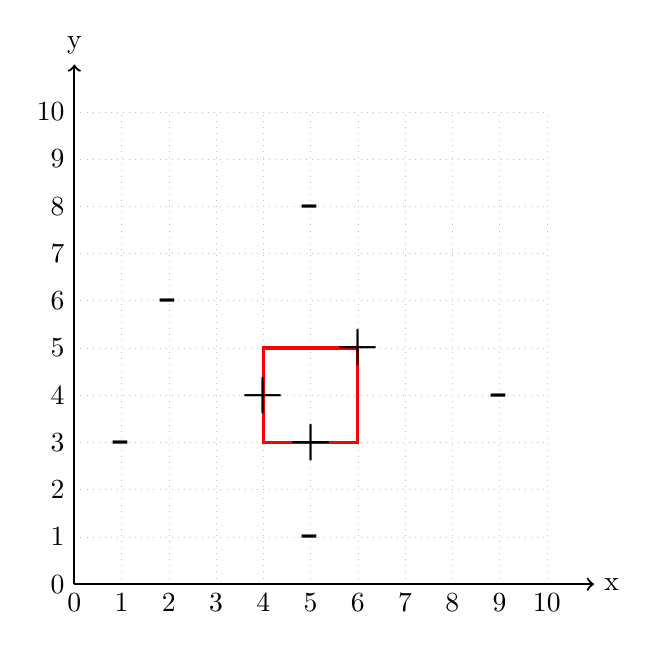
\begin{tikzpicture}[scale=0.6]
								% Draw the grid
								\draw[step=1cm,dotted,gray,very thin,opacity=0.5] (0,0) grid (10,10);
								
								% Label the axes
								\foreach \x in {0,1,...,10} \draw (\x,0) node[below] {\x};
								\foreach \y in {0,1,...,10} \draw (0,\y) node[left] {\y};
								
								% Optionally, draw the x and y axes
								\draw[thick,->] (0,0) -- (11,0) node[right] {x};
								\draw[thick,->] (0,0) -- (0,11) node[above] {y};
								
								% Making rect
								\mkrect[red]{4}{3}{6}{5}
								
								% Mark points with + and -
								\ap{1}{3}{-}
								\ap{2}{6}{-}
								\ap{4}{4}{+}
								\ap{5}{1}{-}
								\ap{5}{3}{+}
								\ap{5}{8}{-}
								\ap{6}{5}{+}	
								\ap{9}{4}{-}
							\end{tikzpicture}
						\end{figure}
			%Q1-b
			\newpage
			\subsection{What is the $G$ boundary of this version space? Write out the hypotheses and
				draw them in.}
			
			% G boundry
			\subsubsection*{Answer:}			
			$$
			G = \{h\}
			$$
			$$
			h: 3 \le x \le 8 ~~ , ~~ 2 \le y \le 7
			$$
			The \textit{blue} rectangle is the $G$ boundary :
			\begin{figure}[h!]
				\centering
				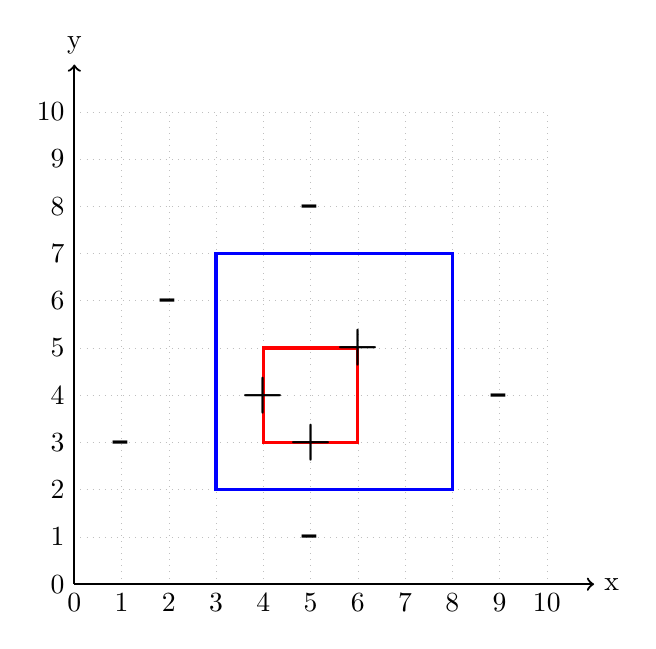
\begin{tikzpicture}[scale=0.6]
					% Draw the grid
					\draw[step=1cm,dotted,gray,very thin,opacity=0.5] (0,0) grid (10,10);
					
					% Label the axes
					\foreach \x in {0,1,...,10} \draw (\x,0) node[below] {\x};
					\foreach \y in {0,1,...,10} \draw (0,\y) node[left] {\y};
					
					% Optionally, draw the x and y axes
					\draw[thick,->] (0,0) -- (11,0) node[right] {x};
					\draw[thick,->] (0,0) -- (0,11) node[above] {y};
					
					% Making rect
					\mkrect[red]{4}{3}{6}{5}
					\mkrect[blue]{3}{2}{8}{7}
					
					% Mark points with + and -
					\ap{1}{3}{-}
					\ap{2}{6}{-}
					\ap{4}{4}{+}
					\ap{5}{1}{-}
					\ap{5}{3}{+}
					\ap{5}{8}{-}
					\ap{6}{5}{+}	
					\ap{9}{4}{-}
				\end{tikzpicture}
			\end{figure}
			
			\subsection{Suppose the learner may now suggest a new $x$ , $y$ instance and ask the trainer for
				its classification. Suggest a query guaranteed to reduce the size of the version space,
				regardless of how the trainer classifies it. Suggest one that will not.}
				
			% G boundry
			\subsubsection*{Answer:}			
			If $P = (7, 4)$ and $+$, then the $S$ boundary will get larger and thus, the size of the version space will get smaller.
			\begin{figure}[h!]
				\centering
				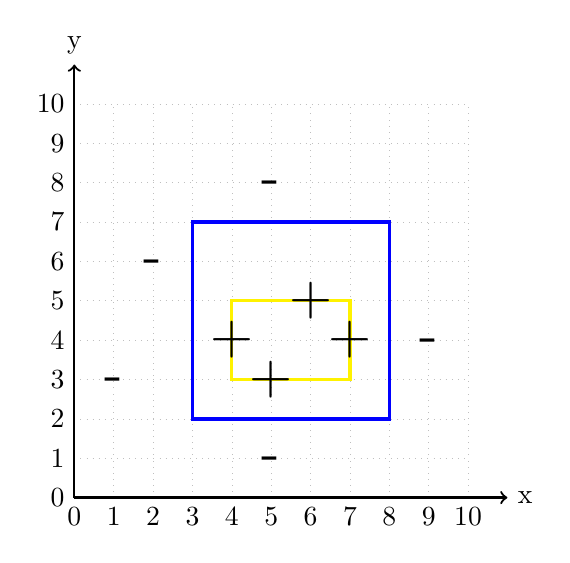
\begin{tikzpicture}[scale=0.5]
					% Draw the grid
					\draw[step=1cm,dotted,gray,very thin,opacity=0.5] (0,0) grid (10,10);
					
					% Label the axes
					\foreach \x in {0,1,...,10} \draw (\x,0) node[below] {\x};
					\foreach \y in {0,1,...,10} \draw (0,\y) node[left] {\y};
					
					% Optionally, draw the x and y axes
					\draw[thick,->] (0,0) -- (11,0) node[right] {x};
					\draw[thick,->] (0,0) -- (0,11) node[above] {y};
					
					% Making rect
					\mkrect[yellow]{4}{3}{7}{5}
					\mkrect[blue]{3}{2}{8}{7}
					
					% Mark points with + and -
					\ap{1}{3}{-}
					\ap{2}{6}{-}
					\ap{4}{4}{+}
					\ap{5}{1}{-}
					\ap{5}{3}{+}
					\ap{5}{8}{-}
					\ap{6}{5}{+}	
					\ap{9}{4}{-}
					\ap{7}{4}{+}
				\end{tikzpicture}
			\end{figure}
			\newpage
			If point $P$ is located outside $G$ boundary and is $-$ (or is $+$ and inside the $S$ boundary), it will not cause any changes to the size of the version space.
			e.g. $P = (2, 9)$
			\begin{figure}[h!]
				\centering
				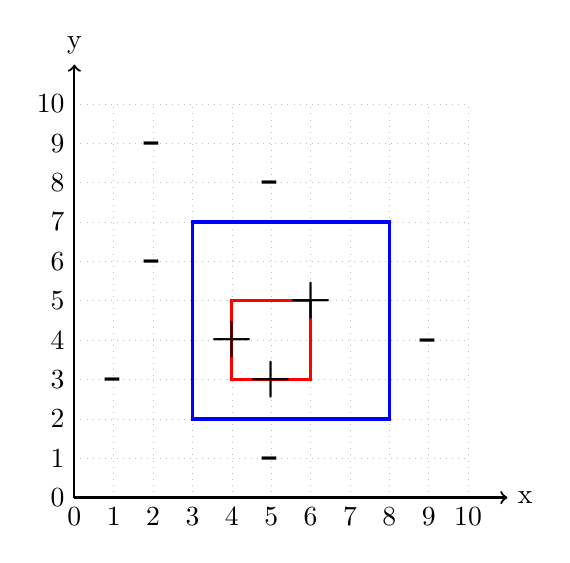
\begin{tikzpicture}[scale=0.5]
					% Draw the grid
					\draw[step=1cm,dotted,gray,very thin,opacity=0.5] (0,0) grid (10,10);
					
					% Label the axes
					\foreach \x in {0,1,...,10} \draw (\x,0) node[below] {\x};
					\foreach \y in {0,1,...,10} \draw (0,\y) node[left] {\y};
					
					% Optionally, draw the x and y axes
					\draw[thick,->] (0,0) -- (11,0) node[right] {x};
					\draw[thick,->] (0,0) -- (0,11) node[above] {y};
					
					% Making rect
					\mkrect[red]{4}{3}{6}{5}
					\mkrect[blue]{3}{2}{8}{7}
					
					% Mark points with + and -
					\ap{1}{3}{-}
					\ap{2}{6}{-}
					\ap{4}{4}{+}
					\ap{5}{1}{-}
					\ap{5}{3}{+}
					\ap{5}{8}{-}
					\ap{6}{5}{+}	
					\ap{9}{4}{-}
					\ap{2}{9}{-}					
				\end{tikzpicture}
			\end{figure}
			
			%Q1-d
			\subsection{Now assume you are a teacher, attempting to teach a particular target concept (e.g.,
				$$
				3 \le x \le 5 , 2 \le y \le 9
				$$
				). What is the smallest number of training examples you can
				provide so that the CANDIDATE-ELIMINATION algorithm will perfectly learn the
				target concept?}
				\subsubsection*{Answer:}
				I believe we need minimally 6 instances, 2 positive and 4 negative examples learn any hypothesis $h$ \textbf{perfectly}.\\
				In order to perfectly learn any hypothesis in this space:
				$$
				\text{Version Space} = \{h\}
				$$
				and for this to happen, $G$ must be equal to $S$:
				$$
				G = S 
				$$
					\begin{figure}[h!]
						\centering
						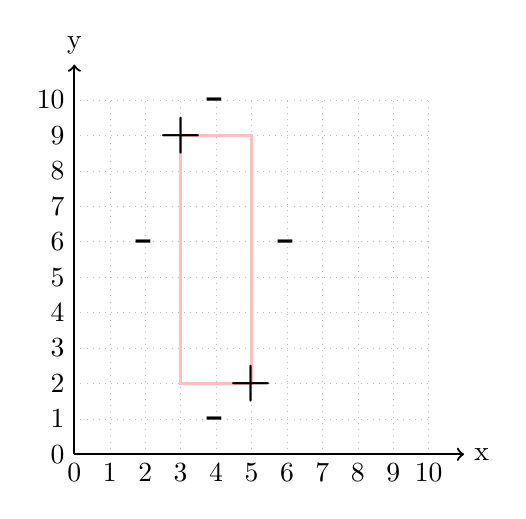
\begin{tikzpicture}[scale=0.45]
							% Draw the grid
							\draw[step=1cm,dotted,gray,very thin,opacity=0.5] (0,0) grid (10,10);
							
							% Label the axes
							\foreach \x in {0,1,...,10} \draw (\x,0) node[below] {\x};
							\foreach \y in {0,1,...,10} \draw (0,\y) node[left] {\y};
							
							% Optionally, draw the x and y axes
							\draw[thick,->] (0,0) -- (11,0) node[right] {x};
							\draw[thick,->] (0,0) -- (0,11) node[above] {y};
							
							% Making rect
							\mkrect[pink]{3}{2}{5}{9}
										
							% Making points
							\ap{3}{9}{+}
							\ap{5}{2}{+}
							\ap{6}{6}{-}
							\ap{2}{6}{-}
							\ap{4}{1}{-}
							\ap{4}{10}{-}
							
						\end{tikzpicture}
					\end{figure}	
	\end{latin}
	
\end{document}